\section{Evaluation}

The goal of our evaluation is to show two main properties of
\textit{ShrinkNets}: they are exploring the space of possible sizes in a "smart"
way, and that as a result we obtain the smaller or equal size than
\textit{Static Networks}. We will then evaluate the performance benefits implied
by these gains in size.

\subsection{Datasets and Setup}

\subsubsection{\texttt{CIFAR10}}

Previous attempt at solving this problem focus on simple datasets and simple
architectures (limited to Fully connected). We believe that self-resizing
network really matter for problems where the architecture you need to solve them
involve so many layers that it is impractical to explore the space of possible
sizes. We considered ImageNet \cite{ILSVRC15} but the time required to train models is so long
that it would have not been possible to train enough and get statistically
significant results. This is why we picked \texttt{CIFAR10} \cite{Krizhevsky2009}. It is an
image classification dataset containing $60000$ color images $(3 \times 32
\times 32)$, belonging to $10$ different classes.

To solve this task we use the \texttt{VGG16} model \cite{Srivastava2014}. It is
constituted of alternating convolutional layers and \textit{MaxPool} layers
interleaved by \textit{BatchNorm} \cite{DBLP:journals/corr/IoffeS15} and
\textit{ReLU} \cite{Nair2010}  layers. The two last layers are Fully connected
layers separated by just a \textit{ReLU} activation function.

To turn it into a ShrinkNet we introduce \textit{Switch Layers} after each
\textit{BatchNorm} and each Fully connected (except the last one).

ShrinkNets assume that the starting size of the network is an upper bound on the
optimal size. We though that picking two times the recommended size for each
layer (that was designed for ImageNet), is a generous upper bound. For the
classification layers we use $5000$ neurons as an upper bound where the ImageNet
version uses $4096$ \gl{This is on the top of my head, need to be double checked}.

We assume no prior knowledge on the optimal batch size, learning rate,
$\lambda$ or weight decay ($\lambda_2$). This is why, we randomly sample them
from a range of reasonable values (\gl{should we make them explicit ?}).
Training is done using our library, based on \texttt{PyTorch} \cite{paszke2017automatic}, that
support dynamically resized layers. We train the network using gradient descent
and \textit{Adam} optimizer \cite{DBLP:journals/corr/KingmaB14}. We start with
the learning rate sampled randomly and every $5$ epochs of non improvement in
validation accuracy we divide the learning rate by $10$. We stop training after
$400$ epochs or when the learning rate is under $10^{-7}$ whichever comes
first. \gl{Should I also give the details about the removal strategy we used
  and the $\gamma$ and threshold I used ? because this is clearly getting
  boring} For each of the models we trained, we pick the epoch with the best
validation accuracy and report the corresponding testing accuracy. Because of
the nature of our method, it can happen that for network that are aggressively
compressed, the best validation accuracy is obtained early in the training,
before the size has converged. To be sure that accuracy measured corresponds to
the final shape and not the starting shape, we only consider the second half of
the training when picking the best epoch. For each model, we also measure the
total size, in number of floating point parameters, excluding the
\textit{Switch Layers} because as we saw in \cref{neuron_killing}, we can
get rid of them when training is done.

We want to compare against classical (\textit{Static}) networks. The number of
parameters that control the size is large: 13 for the size of convolutional
layers and $2$ for the fully connected ones. Without Shrinknets to help and fuse
all these parameters in a single $\lambda$ it is infeasible to sample reasonably
well a search space of that size. This is why we have to rely on the very well
known heuristic that the original VGG architecture (and many CNNs) \gl{try to
  find the paper that introduces this heuristic}. For \textit{Static Networks}
we sample the size between $0.1$ and $2$ times the size optimized for ImageNet.
We report the same numbers as we did for \textit{ShrinkNets} and we compare the
two distributions of models we obtain on the first plot of \cref{figure_CIFAR10}.


\subsubsection{\texttt{COVERTYPE} dataset}

Our second dataset we will evaluate on is \texttt{COVERTYPE} \cite{Blackard:1998:CNN:928509}. This dataset
contains $581012$ description of geographical area (elevation, inclination,
etc...) and the goal is to predict the type of forest growing there. We picked
this one for couple of reasons. First it is simple that we can reach good
accuracy with only a few layers. This important because we want to show that
\textit{ShrinkNets} find sizes as good as \textit{Static Networks}, even if we
are sampling the entire space of possible sizes. The second reason is that [ref]
also perform their evaluation on this dataset, which allow us to compare the
results obtained by the two methods.

The only difference in terms of setup are minimal. We use the same architecture
as \cite{Scardapane2017}, i.e. three layers Fully Connected neural network with  no
\textit{Dropout} \cite{Srivastava2014} nor \textit{BatchNorm}. \gl{Should we say here that we
  don't expect Dropout to work here ? I could write an entire paragraph about it
  if needed}. In this case for the \textit{Static Networks}, we sample
independently sizes of the three different layers to explore all possible
architectures.

\subsection{Results of the random search procedure}

On the plot, the Pareto front for the two training methods clearly indicates
that not only \textit{ShrinkNets} find models that are as accurate as
\textit{Static Networks}, but they are more efficient in terms of size. Even
when we sample the entire size space (in the \texttt{COVERTYPE} case),
\textit{ShrinkNets} are better or equally as good as \textit{Static Networks}.
it has two implications. First it reinforces, our observation in [ref] that
showed that the models do not suffer from the non-convexity introduced by the
multiplication by the \textit{Switch Layer}. Secondly it could let us conjecture
that the parametrization from a $\lambda$ (real value) to the size of the
size of the network (vector) close to optimal. Indeed, if it was
not the case then eventually a randomly sampled size would have beaten
\textit{ShrinkNets} models. \gl{Too strong ?}

\subsection{Benefits of smaller sizes}

We showed in the previous section that \textit{ShrinkNets} were able to find
more or at least as efficient as \textit{Static Networks}. In this experiment we
want to determine benefits of the smaller size we get.

For some applications, the absolute best accuracy is not something desirable if
it implies having enormous models. This observation motivates our methodology:
for a given target accuracy that you want your model to achieve, we pick the
smallest that satisfy the constraint. For both \textit{ShrinkNets} and
\textit{Static Networks} we measure multiple metrics and compute the ratio
between the two. The metrics are interested in are: the final model size (in
number of parameters) and inference speed on CPU and GPU for small batch sizes
($1$ input) and large batch sizes (depend on the dataset and hardware). Results
are shown on \cref{figure_CIFAR10} and \cref{figure_COVER} after the
distribution of sizes and accuracy. We limit our plot to the ($80-100\%$
accuracy range because we consider that models with lower accuracy have less
practical use).

Regarding size, the key observation we can make is that size improvenets are
significant for the \texttt{CIFAR10}. In the range of accuracies we are
interested in, improvements in size go from 4x to 40x. On the \texttt{COVERTYPE}
dataset even if the compression ratio is always above 1, it hardly exceeds 3x,
except for very high accuracy where \textit{ShrinkNets} obtained some
particularly good solutions.

We observe that unlike local sparsity compression based method, our method
translates directly improvement in size to higher bandwidth at inference time.
In situations where inference is already incredibly fast (\texttt{COVERTYPE}
with a batch size of $1$ and \texttt{CIFAR10} with a batch size of $1$ on GPU),
improvements are dominted by noise. However, on machine learning frameworks
more focused on latency it should be possible to measure them.


% \begin{figure}
% \begin{center}
% 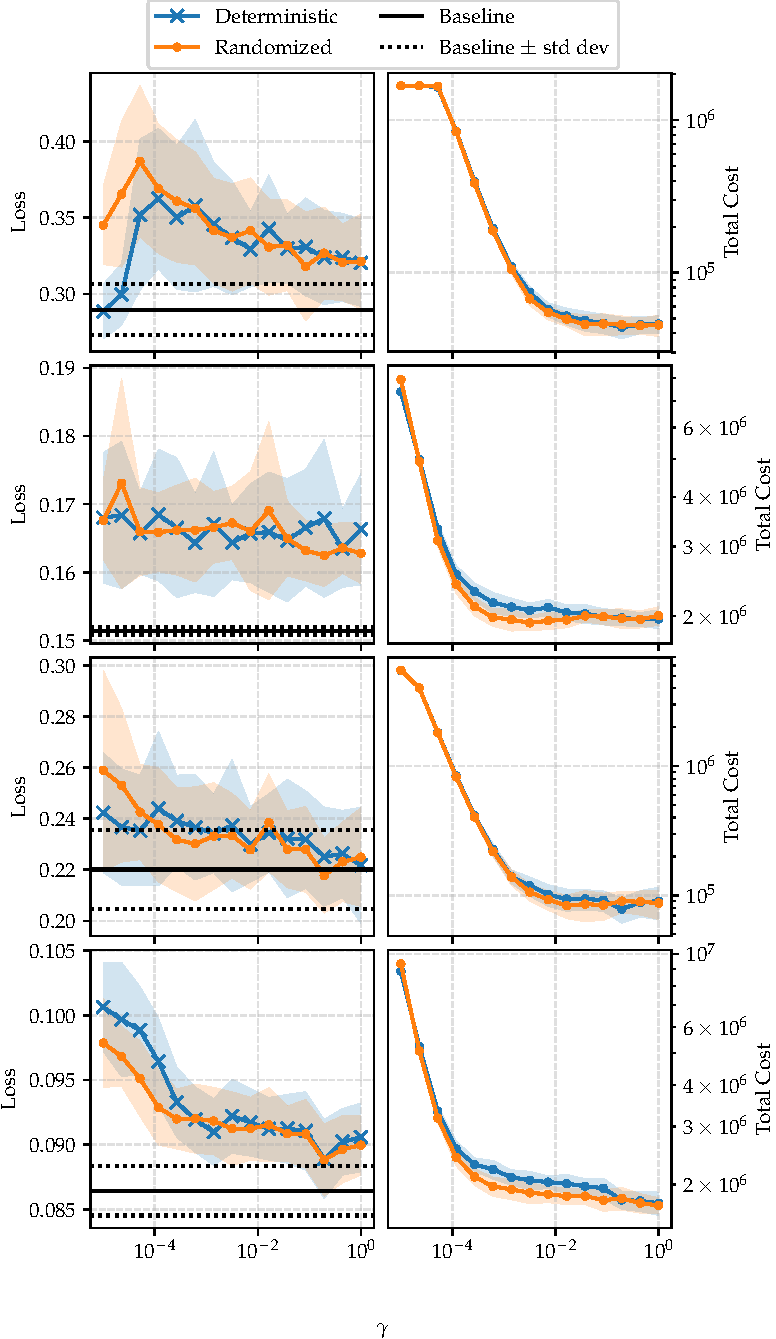
\includegraphics[width=\columnwidth]{neuron_removal}
% \vspace*{-5mm}
% \caption{\label{neuron_removal_figure}Effect of dynamic neuron removal for different $\gamma$. First column is the difference in the final loss in function of the removal factor. We plot theoretical baseline as a reference. Right column is a proxy of the total cost for training the model (i.e. the sum of input neurons at each epoch). Each row is a dataset/$\lambda$ combination. From top to bottom we have: \texttt{scm1d}/$0.1$, \texttt{oes97}/$0.1$}
% 
% \end{center}
% \vspace*{-4mm}
% \end{figure}

\begin{figure}
\begin{center}
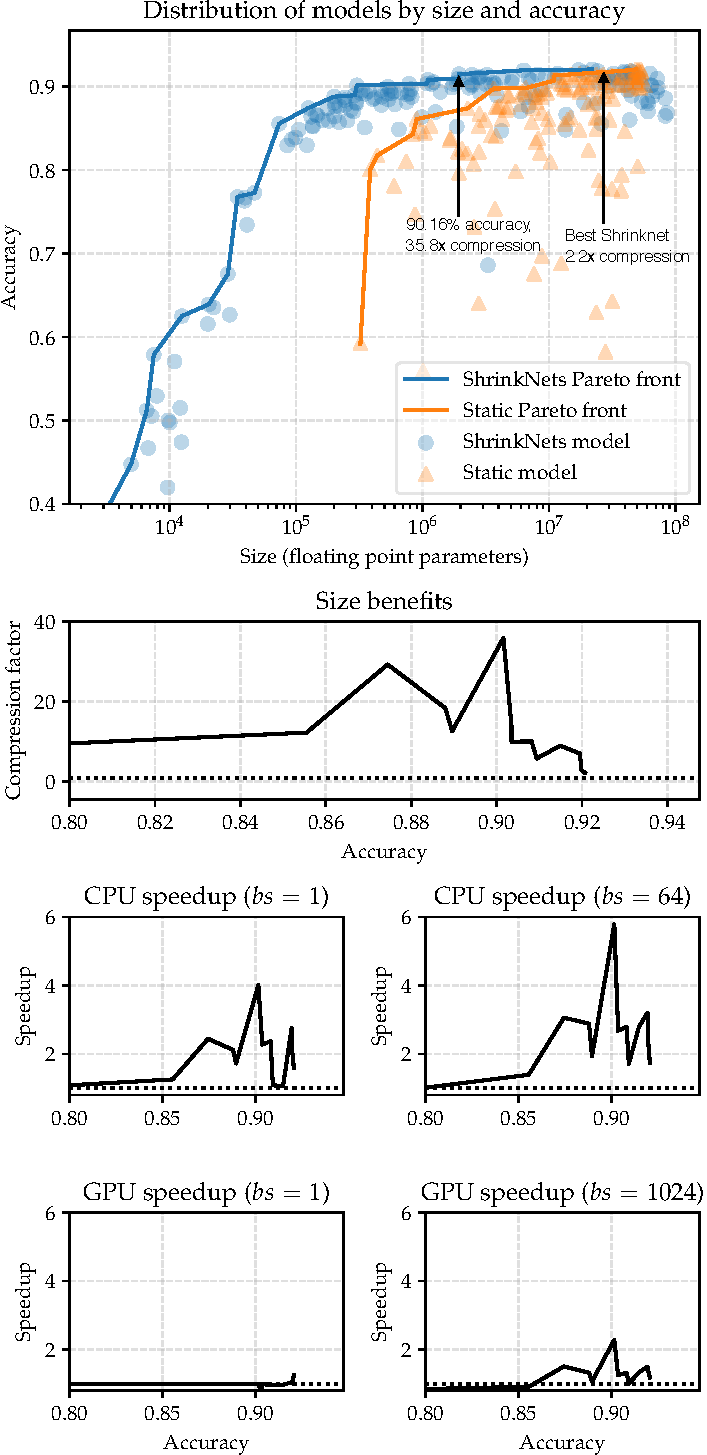
\includegraphics[width=\columnwidth]{CIFAR10_VGG_summary}
\vspace*{-5mm}
\caption{\label{figure_CIFAR10} Summary of the result of random
search over the hyper-parameters the \texttt{CIFAR10} dataset}
\end{center}
\vspace*{-4mm}
\end{figure}

\begin{figure}
\begin{center}
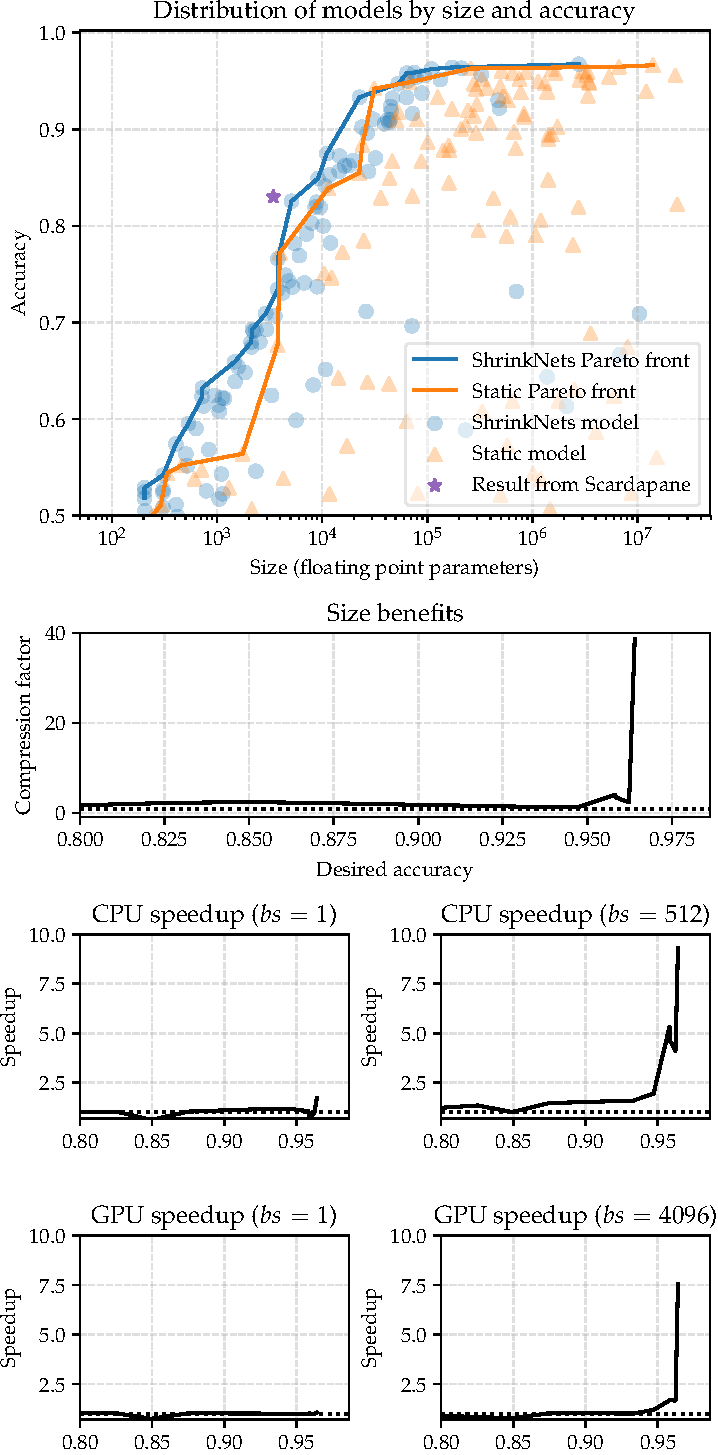
\includegraphics[width=\columnwidth]{COVER_FC_summary}
\vspace*{-5mm}
\caption{\label{figure_COVER} Summary of the result of random
search over the hyper-parameters the \texttt{COVERTYPE} dataset}
\end{center}
\vspace*{-4mm}
\end{figure}


\subsection{Architectures obtained after convergence}

We sucessfully demonstrated that the architecture \textit{Shrinknets} converge
to make sense both in term of size and performance. And for a given accuracy
the size needed is significantly smaller than when we use the classic heursitc
we commonly use to size convolutional neural networks. It might be an
indication that this strategy is suboptimal and might need to be adjusted.
During our experimentations on simpler datasets like \texttt{MNIST}
\cite{Lecun1998} and \texttt{FashionMNIST} \cite{Xiao2017} we observed that
even if they have the same number of classes, input features, and output
distribution. For a fixed $\lambda$ \textit{ShrinkNets} converged to
considerably bigger networks in the case of \texttt{FashionMNIST}. This
evidence shows that final architecture not only depends on the output
distribution or shape of the data but actually reflects the dataset, indeed we
know that \texttt{MNIST} is a much easier problem than \texttt{FashionMNIST}.

We provide two examples of architectures learned by \textit{ShrinkNet}. One
for the best test available test accuracy and a slightly underperforming but
significantly smaller that it's equivalent \textit{Static Network}. For
these two architectures we show the size at different time during training to
give a sense how the convergence happen.

\begin{figure}
\begin{center}
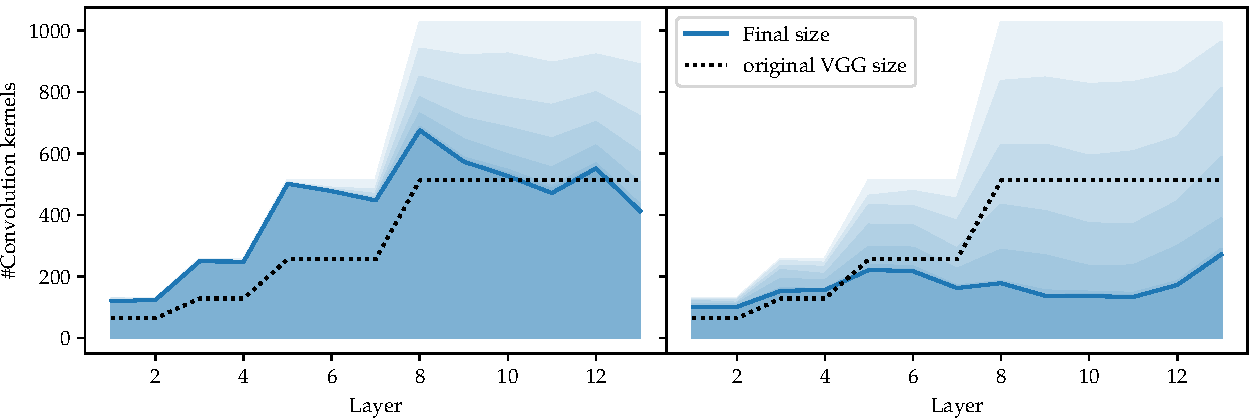
\includegraphics[width=\columnwidth]{size_evolution}
\vspace*{-5mm} \caption{\label{network_size_evolution} Evolution of the size of
  each layer over time (lighter: beginning, darker: end). On top a very large
  network performing $92.07\%$, at the bottom a simpler model with $90.5\%$
  accuracy
} \end{center}
\vspace*{-4mm}
\end{figure}

% \subsection{Neuron Removal strategies [TO be removed]}
% 
% In our previous experiment, we showed that the ShrinkNet loss was
% reasonable in practice, we are now interested in the impact on
% early pruning. The method we suggest for early prunning uses a
% parameter $\gamma$ that control the aggressiveness of neuron removal
% so we will try to evaluate its impact on the final loss achieved by
% the model and the cost required to train the model. Our cost model
% is simple and hardware independant, we sum the number of input neurons
% at each epoch. In theory the cost in time should be asymptotically
% linear to this metric. To have a baseline we also train the same model
% but without neuron removal. Keep in mind that this is just in order to
% have some reference. Indeed, if we were to remove the neurons with small
% weights it would deteriorate the loss (and picking the threshould would
% be completely arbitrary). Therefore the baseline is evaluated with all neurons.
% One could consider it as a "theoretical lower bound" of the best achievable loss.
% 
% 
% We picked multiple combinations of dataset and regularization parameters ($\lambda$) and for each we fit with different aggressiveness parameters ($\gamma$). We measure the loss after convergence and the total cost and report the result in \cref{neuron_removal_figure}. In order to reduce the noise in the result, each experiment was performed $30$ times and we display the range arround $\pm$ $1$ standard deviation.